% use paper, or submit
% use 11 pt (preferred), 12 pt, or 10 pt only

\documentclass[letterpaper, preprint, paper,11pt]{AAS}	% for preprint proceedings
%\documentclass[letterpaper, paper,11pt]{AAS}		% for final proceedings (20-page limit)
%\documentclass[letterpaper, paper,12pt]{AAS}		% for final proceedings (20-page limit)
%\documentclass[letterpaper, paper,10pt]{AAS}		% for final proceedings (20-page limit)
%\documentclass[letterpaper, submit]{AAS}			% to submit to JAS

\usepackage{bm}
\usepackage{amsmath}
\usepackage{subfigure}
%\usepackage[notref,notcite]{showkeys}  % use this to temporarily show labels
\usepackage[colorlinks=true, pdfstartview=FitV, linkcolor=black, citecolor= black, urlcolor= black]{hyperref}
\usepackage{overcite}
\usepackage{footnpag}			      	% make footnote symbols restart on each page




\PaperNumber{XX-XXX}



\begin{document}

\title{MANUSCRIPT TITLE (UP TO 6 INCHES IN WIDTH AND CENTERED, 14 POINT BOLD FONT, MAJUSCULE)}

\author{John L. Doe\thanks{Title, department, affiliation, postal address.},  
Jane Roe\thanks{Title, department, affiliation, postal address.},
\ and J.Q. Public\thanks{Title, department, affiliation, postal address.}
}


\maketitle{} 		


\begin{abstract}
The abstract should briefly state the purpose of the manuscript, the problem to be addressed, the approach taken, and the nature of results or conclusions that can be expected. It should stand independently and tell enough about the manuscript to permit the reader to decide whether the subject is of specific interest. The abstract shall be typed single space, justified, centered, and with a column width of 4.5 inches. The abstract is not preceded by a heading of ``Abstract'' and its length may not extend beyond the first page.
\end{abstract}








\section{Introduction}
The American Astronautical Society (AAS) publishes bound sets of printed conference proceedings for personal, institutional, and library usage. The availability of hardcopy enhances the longevity of your work and elevates the importance of your conference contribution to professionals through archival publication. To preserve the consistency and quality of the proceedings, all authors adhere to the latest version of AAS conference proceedings format.


This document is intended to serve as a visual and instructional guide, and as a \LaTeX\ document template, for the AAS conference proceedings format. This template provides the basic font sizes, styles, and margins required by the publisher's formatting instructions.   There are also styles for centered equations, figure and table captions, section and sub-section headings, footnote text, \emph{etc}. This template provides samples of their usage.  To use this document as a template, simply copy and change its contents with your own information while maintaining the required predefined style, rather than starting anew. Since this is not a tutorial on how to use \LaTeX\, refer to \LaTeX\ manuals for more information.


Your manuscript should include a paper number, a title, an author listing, an abstract, an introductory section, one or more sections containing the main body of the manuscript, a concluding summary section, and a reference or bibliography section. You may also include a section on notation, an acknowledgements section, and appendices, as illustrated in the sequel. You should \emph{not} include a leading cover sheet. Author affiliation shall appear on the first page, added as a footnote to the last name of each the author. If a distributional release statement or copyright notice is required by your sponsor, this is added as a footnote to the title of the manuscript, appearing on the first page only. Page numbers should be centered halfway between the lower margin and the bottom edge of the page (\emph{i.e.}, approximately 0.75 inches from the bottom). Copy should be single space with double space between paragraphs, with the first line of each paragraph indented 0.2 inches.

The recommended sans-serif font for paper number, title, and author listing is \emph{Arial}, or, \emph{Helvetica}. The title font and paper-number font should be the same: 14-point sans-serif, centered, and bold. The author-listing font should be 12-point sans-serif, centered, and bold. The recommended serif font for body text, headings, \emph{etc}., is \emph{Times} or \emph{Times New Roman} at 10-12 point, 11 point preferred. The captions for figures and tables are bold 10-point serif font. The endnote reference text and footnote text is 9-point serif font. The right-hand margin of body text should be justified; if not, it should be fairly even nevertheless. All text and text background shall remain uncolored (black on white). These conventions should be automatically implemented in this \LaTeX\ template when the predefined styles of this template are used.

The body text of this template is based on the preferred font size of 11 points. To change this to 12-point size, increase the font size at the top of the \LaTeX\ template by uncommenting the appropriate {\tt documentclass[]\{\}} line. For very long manuscripts, a 10-point font may be used to keep the manuscript within the publisher's limit of twenty (20) physical pages.


\section{This is a Sample of a General Section Heading}
Numbering of section headings and paragraphs should be avoided. Major section headings are majuscule, bold, flush (aligned) left, and use the same style san-serif font as the body text. Widow and orphan lines should also be avoided; more than one line of a paragraph should appear at the end or beginning of a page, not one line by itself. A heading should not appear at the bottom of a page without at least two lines of text. Equations, figures, and tables must be sequentially numbered with no repeated numbers or gaps. Excessive white space --- such as large gaps before, between, and after text and figures --- should be minimal and eliminated where possible.





\subsection{This Is a Sample of a Secondary (Sub-Section) Heading}
Secondary, or sub-section, headings are title case (miniscule lettering with the first letter of major words majuscule), flush left, and bold. Secondary headings use the same serif font style as the body text and, like section headings, should not be numbered. Tertiary headings should be avoided, but if necessary, they are run-in, italic, and end in a period, as illustrated with the next six (6) paragraphs.
\begin{equation}
	\label{eq:ab}
	a = b^{2}
\end{equation}

\subsubsection{Equations.} 
Equations are centered with the equation number flush to the right. In the text, these equations should be referenced by name as Eq.~\eqref{eq:ab} or Equation~\eqref{eq:ab} (\emph{e.g}., not eq. 1, (1), or \emph{Equation 1}). To improve readability, scalar variable names such as $a$ and $b^{2}$ are usually italicized when appearing in text and equations.\footnote{A section on mathematical notation is provided in the sequel.}



\subsubsection{Abbreviations.} 
When abbreviations for units of measure are used, lower case without periods is preferred in most instances; \emph{e.g}. ft, yd, sec, ft/sec, \emph{etc}., but in. for inch.




\begin{figure}[htb]
	\centering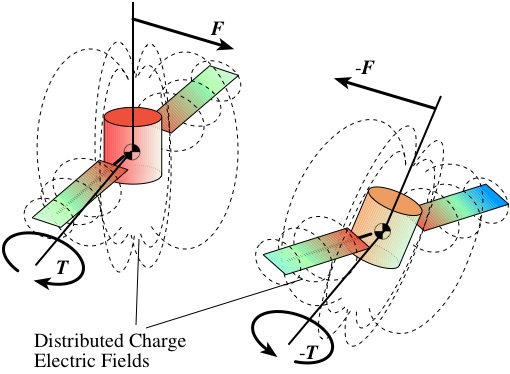
\includegraphics[width=3.5in]{Figures/test}
	\caption{Illustration Caption Goes Here}
	\label{fig:xxx}
\end{figure}

\subsubsection{Figures.}   
Illustrations are referenced by name and without formatting embellishments, such as Figure~\ref{fig:xxx}, Figure 2, \emph{etc}., or, Figures 3 and 4 (\emph{e.g}., not figure (1), Fig. 1, \underline{Figure 1}, \emph{Figure 1}, \emph{etc}.). Each illustration should have a caption unless it is a mere sketch. Single-phrase captions are usually in title case; they are bold 10-point serif font and centered below the figure as shown in Figure~\ref{fig:xxx}. An explanatory caption of several sentences is permissible. Ideally, every illustration should be legibly sized -- usually about one-half or one-quarter page -- and appear in the text just before it is called out or mentioned. Alternatively, it is also permissible to place all figures together at the end of the text as a separate appendix; however, these two conventions should not be mixed. All figures and callouts should remain clearly legible after reduction. All illustrations appear as black and white in the final printing, although colors are retained in the electronic (CD-ROM) version.


\subsubsection{Graphic Formats.} 
The highest quality formats are Encapsulated PostScript (EPS) and PDF vector-graphic formats. These formats are recommended for all illustrations, unless they create document files that are excessively large. Specifically, you should change the graphic format or compress the image resolution whenever an illustrated page takes more than two seconds to render onscreen, or, whenever the total manuscript file size starts to approach 5 Mb. Photographs, illustrations that use heavy toner or ink (such as bar graphs), and figures without text callouts, may be suitably displayed with picture formats such as BMP, GIF, JPEG, PNG, TIFF, \emph{etc}. Line drawings, plots, and callouts on illustrations, should not use picture formats that do not provide sharp reproduction. All graphical content must be embedded when creating a PDF document, especially any fonts used within the illustration. Note that the Windows Metafile Format (WMF) is sometimes problematic and should be avoided.


\subsubsection{References and Citations.} 
The citation of bibliographical endnote references is indicated in the text by superscripted Arabic numerals, preferably at the end of a sentence.\cite{doe2005, style1959}   If this citation causes confusion in mathematics, or if a superscript is inappropriate for other reasons, this may be alternately expressed as (Reference~\citenum{doe2005}) or (see References~\citenum{doe2005} and \citenum{style1959}), (\emph{e.g}., not [1], Ref. (1), \emph{etc}.). While there is no singly prescribed format for every bibliographical endnote, references should be consistent in form. Citations should be sufficient to allow the reader to precisely find the information being cited, and should include specific pages, editions, and printing numbers where necessary. URL citations are discouraged, especially when an archival source for the same information is available. If a URL citation is required, it should appear completely and as a footnote instead of a bibliographical reference.\footnote{\url{http://www.univelt.com/FAQ.html\#SUBMISSION}}  The citation of private communication is especially discouraged, but if required it should be cited as a footnote and include the date, professional affiliation, and location of the person cited.\footnote{Gangster, Maurice (1999), personal correspondence of March 21st. Sr. Consultant, Space Cowboy Associates, Inc., Colorado Springs, CO.}  



\begin{table}[htbp]
	\fontsize{10}{10}\selectfont
    \caption{A Caption Goes Here}
   \label{tab:label}
        \centering 
   \begin{tabular}{c | r | r } % Column formatting, 
      \hline 
      Animal    & Description & Price (\$)\\
      \hline 
      Gnat      & per gram & 13.65 \\
                & each     &  0.01 \\
      Gnu       & stuffed  & 92.50 \\
      Emu       & stuffed  & 33.33 \\
      Armadillo & frozen   &  8.99 \\
      \hline
   \end{tabular}
\end{table}

\emph{Tables.} 
Tables are referred to by name in the text as Table~\ref{tab:label}, or, Tables 2 and 3 (\emph{e.g}., not table 1, Tbl. 1, or \emph{Table 1}). The title is centered above the table, as shown in Table 1. The font size inside tables should be no larger than the body text, but may be adjusted down to 9-point if necessary (10-point serif font is considered nominal). Note that table units are in parentheses. Only the minimum number of table lines needed for clarity is desired. Ideally, every table should appear within the text just before it is called out, but, it is also permissible to place all tables together at the end of the text as a separate appendix. If so, these two conventions should not be mixed.

Equations, figures, and tables must be sequentially numbered with no repeated numbers or gaps. Each figure and table shall be called out in the text; gratuitous figures and tables that are not called out should be eliminated. Intermediate equations may be numbered without being called out.




\section{Manuscript Submission}
The Portable Document Format (PDF) is the preferred format for electronic submissions.\footnote{By contributing your manuscript for proceedings publication, you necessarily extend any copyrights to the AAS and its designated publisher, to allow the AAS to publish your manuscript content in all the forms that it wishes.}
 The page size should be 8.5 inches by 11 inches exactly. You should use ``press-quality'' or ``high-quality'' software settings to create your PDF file; these settings tend to keep the PDF file true to the original manuscript layout, and automatically embed the correct fonts, \emph{etc}. Otherwise, settings such as ``Embed All Fonts'', \emph{etc}., should be selected as available. The use of internal hyperlinks within the electronic file is not encouraged because hyperlinks may not be supported in the final version of the electronic proceedings.

\subsection{Journal Submission}
If you wish to submit this manuscript to the \emph{Journal of Astronautical Sciences}, it must be re-formatted into a double-spaced format. This can be done easily with this template. At the top of the document, there are two (2) types document class statements ({\tt paper} and {\tt submit}).  The first type is the one to use for a conference paper.  The second type , which is commented out, can be used to reformat the paper for the JAS journal submission.


\section{Conclusion}
Some AAS meetings are co-sponsored with the American Institute of Aeronautics and Astronautics (AIAA). When your paper number starts with ``AAS'', or when the conference is described as a joint ``AAS/AIAA'' meeting with the AAS listed first, this AAS conference proceedings format shall be used.

Your final manuscript should be camera-ready as submitted --- free from technical, typographical, and formatting errors. Manuscripts not suitable for publication are omitted from the final proceedings.


\section{Acknowledgment}
Any acknowledgments by the author may appear here. The acknowledgments section is optional.






\section{Notation}
\begin{tabular}{r l}
	$a$ & a real number \\
	$b$ &  the square root of $a$ \\
\end{tabular} \\

If extensive use of mathematical symbols requires a table of notation, that table may appear here. Where the first mathematical symbol is introduced, a footnote should direct the attention of the reader to this table.\footnote{The footnote symbols are a standard sequence: $\ast$, $\dagger$, $\ddag$, \emph{etc}. This sequence of footnote symbols should restart with each new page.}  The notation table should be simple and reasonably consistent with the standards of modern technical journals, as illustrated above. The notation table does not need its own caption like an ordinary table, since the section heading serves this purpose. The notation section is optional.





\appendix
\section*{Appendix: Title here}
Each appendix is its own section with its own section heading. The title of each appendix section is preceded by ``APPENDIX: '' as illustrated above, or ``APPENDIX A: '', ``APPENDIX B: '', \emph{etc}., when multiple appendixes are necessary. Appendices are optional and normally go after references; however, appendices may go ahead of the references section whenever the word processor forces superscripted endnotes to the very end of the document. The contents of each appendix must be called out at least once in the body of the manuscript.


\subsection*{Miscellaneous Physical Dimensions}
The page size shall be the American standard of 8.5 inches by 11 inches (216 mm x 279 mm). Margins are as follows: Top -- 0.75 inch (19 mm); Bottom -- 1.5 inches (38 mm); Left -- 1.25 inches (32 mm); Right -- 1.25 inch (32 mm). The title of the manuscript starts one inch (25.4 mm) below the top margin. Column width is 6 inches (152.5 mm) and column length is 8.75 inches (222.5 mm). The abstract is 4.5 inches (114 mm) in width, centered, justified, 10 point normal (serif) font.


\bibliographystyle{AAS_publication}   % Number the references.
\bibliography{references}   % Use references.bib to resolve the labels.



\end{document}
